\section{Empirical Study}
\label{sec:evaluation}
We seek to answer the following five research questions (RQs) through our experimental evaluation.
\begin{itemize}
    \item\underline{\textbf{RQ1}}: Are our proposed data structures practical for large scale VNFPPs?
    \item\underline{\textbf{RQ2}}: Does our new initialization operator improve upon our previous operator?
    \item\underline{\textbf{RQ3}}: How does our proposed metaheuristic compare against other parallel and synchronous MOEAs?
    \item\underline{\textbf{RQ4}}: Does our proposed heuristic objective function improve on existing objective functions?
    \item\underline{\textbf{RQ5}}: What are the largest problem instances we can consider and what are the current limiting factors?
\end{itemize}

For each research question, we consider three common network topologies: DCell \cite{GuoWTSZL08}, Fat Tree \cite{Al-FaresLV08}, and Leaf-Spine \cite{Cisco19}, illustrated in \pref{fig:topologies}. Where applicable, we calculate the HV of populations of solutions to judge the convergence and diversity of the population. Due to the disparity in the objectives, in each of these tests we first normalize the objective values of all solutions as described in the appendix. The parameter settings for each algorithm are based on the respective authors' recommendations and are also listed in the appendix.

\begin{table}[t]
    \caption{Category and actual number of servers for each network topology}
    \label{tbl:scales}

    \centering
    \begin{tabularx}{\linewidth}{lXXX}
        \toprule
        \multirow{2}{6em}{Number of servers} & \multicolumn{3}{c}{Topology}                      \\
        \cmidrule{2-4}
                                             & Fat Tree                     & Leaf-Spine & DCell \\
        \midrule
        500                                  & 423                          & 512        & 420   \\
        1000                                 & 1024                         & 968        & 930   \\
        2000                                 & 2000                         & 2048       & 1806  \\
        4000                                 & 3456                         & 4050       & 3192  \\
        8000                                 & 8192                         & 7938       & 8190  \\
        16000                                & 16000                        & 15842      & 17556 \\
        32000                                & 35152                        & 31752      & 33306 \\
        64000                                & 65536                        & 64082      & 57840 \\
        \bottomrule
    \end{tabularx}
\end{table}

\subsection{Distance Table Compression Evaluation}
\label{sec:distance_compression}

\begin{figure*}[t!]
    \centering
    \includegraphics[width=\linewidth]{figures/graphs/distance_table/distance_tables}

    \caption{The minimum setting of $N^T$ that was required to reach 99.9\% reliability.}
    \label{fig:distance_compression_alpha}
\end{figure*}

\subsubsection{Methods}
We first aim to determine the minimum practical size of the distance tables. We use monte-carlo methods to find a minimum acceptable size of the distance tables $N^T$. Smaller settings of $N^T$ will grant larger memory savings but also reduce the probability of finding a feasible placement for all VNFs of all services in a solution. We defined an acceptable setting of $N^T$ as one which will place all service instances for $99.9\%$ of a diverse set of solutions where each solution requires at least 90\% data center utilization. Since it is unlikely that a data center will reach this level of utilization, this ensures that the parameter setting is robust against all but the most extreme situations. Similarly, the 99.9\% threshold ensures that on average most initial solutions in a population will be feasible, reducing the risk of a bias towards solutions with low numbers of VNFs.

We considered three topologies at increasingly large scales. Due to the structure of each network topology, it is not possible for all topologies to have the same number of servers at each scale. The exact number of servers for each scale are listed in \pref{tbl:scales}.

For each data center topology and scale, we defined 100 problem instances and generated 1000 solutions for each problem. For both the stochastic BFS and the deterministic BFS, we found the minimum acceptable setting of $N^T$ in the range $0, 1, \cdots, 100$ (i.e. for $99900/100000$ solutions, all service instances must be placed). Note that lower settings of $N^T$ directly correlate with lower memory consumption e.g., $N^T = 0.2$ indicates an 80\% memory saving compared to the naive method.

\subsubsection{Results}
\pref{fig:distance_compression_alpha} shows the minimum acceptable setting of $\alpha$ for each method and for each topology at each scale. These figures show that the memory requirements of the distance tables can be greatly reduced by utilizing a low setting of $N^T$.

Notably, lower settings of $N^T$ can be tolerated on larger graphs. On the smallest topologies, we found that at least 70\% of the information contained in the naive routing tables was not required. On the largest topologies, typically 99\% of the information is not required. Further, we find that across topologies of each scale, the memory requirements remain fairly constant. This suggests that the \textit{relative percentage} of servers in each distance table is less important than the \textit{number} of servers. It is plausible that there exists a constant value for the size of each distance table for an acceptable feasible solution probability. Given the memory requirements of each distance table can be made satisfactorily small with the existing approach, we leave further exploration of this outcome to future work.

Additionally, we found that our proposed stochastic BFS typically allowed for lower settings of $N^T$ than the traditional deterministic BFS. The DCell topology is a special case where the deterministic BFS outperformed the stochastic BFS, however we note that this does not indicate that the deterministic BFS is preferable. Our implementation of the deterministic BFS first explores the servers which reside under a separate switch. Since the DCell topology is symmetrical, this ensures that each server appears the same number of times, provided that a small enough setting of $N^T$ is used. If a larger size were used, or if the deterministic BFS were instead to explore the local switch first, the non-deterministic BFS would be preferable since in the deterministic BFS a small number of servers would be overrepresented. In this way, the deterministic BFS is only preferable for specific instances that can only be guaranteed to occur when the topology is known. Hence it is not appropriate for arbitrary graphs.

In partial response to RQ1, the effectiveness of our proposed distance table compression algorithm enables us to consider far larger problem instances of all topologies.

\subsection{Routing Table Compression Evaluation}
\label{sec:routing_compression}

\subsubsection{Methods}
Without compression, the routing tables required for the mapping process can require impractical amounts of memory. To determine whether compression can reduce the memory requirements to a practical level, we constructed routing tables with and without compression for each topology and at different scales.

\subsubsection{Results}

\begin{figure*}[t!]
    \centering
    \includegraphics[width=\linewidth]{figures/graphs/routing_table/routing_tables}

    \caption{The comparative memory consumption of the routing tables with and without our proposed compression strategy.}
    \label{fig:rt_compression}
\end{figure*}

\begin{table}[t]
    \caption{The percentage of memory saved by using our compressed routing table.}
    \label{tbl:percent_memory}

    \centering
    \begin{tabularx}{\linewidth}{lXXX}
        \toprule
        \multirow{2}{6em}{Number of servers} & \multicolumn{3}{c}{Topology}                      \\
        \cmidrule{2-4}
                                             & Fat Tree                     & Leaf-Spine & DCell \\
        \midrule
        500                                  & 98.38                        & 98.63      & 24.68 \\
        1000                                 & 99.28                        & 99.26      & 31.00 \\
        2000                                 & 99.61                        & 99.65      & 36.53 \\
        4000                                 & 99.77                        & 99.82      & 41.26 \\
        8000                                 & 99.90                        & 99.91      & 48.84 \\
        16000                                & 99.95                        & 99.95      & 54.67 \\
        32000                                & 99.98                        & 99.98      & 59.31 \\
        64000                                & 99.99                        & 99.99      & 63.10 \\
        \bottomrule
    \end{tabularx}
\end{table}

\pref{fig:rt_compression} shows the amount of memory that the routing tables of each topology required with and without compression. The figure shows how the uncompressed routing tables are impractical for large data centers and also that our proposed compression technique uses significantly less memory than the naive approach.

The routing table compression was most effective on hierarchical data centers, e.g. the Fat Tree and Leaf-Spine topologies. We found that hierarchical topologies are particularly amenable to compression. When all servers communicate with other servers via a switch, all paths for a server can be compressed into 2 or 3 rows (the servers with IDs less than the current server, the current server, and the servers with IDs after the current server). Similarly, the hierarchy of the topology ensures that each port of a switch will allow access to either a single server or a cluster of sequential servers which can be compressed into one row. As a consequence, the compressed routing tables used $\sim$3 orders of magnitude less memory than the uncompressed routing tables.

The compressed DCell routing tables also required significantly less memory, specifically 44.92\% less memory on average (see \pref{tbl:percent_memory}), but still required on the order of 10 - 100 GBs of memory to store the larger topologies. This is because of two related factors. First, the DCell topology uses direct connections between servers. As a consequence, each server requires at least one row for each port. Further, the direct server connections mean that although many servers may be accessed via the same component, the IDs of these servers are only contiguous for short stretches, and hence our compression is less effective. Despite these limitations, the compressed DCell topology still uses significantly fewer rows. Second, each row in our compressed formulation requires 50\% more memory. Specifically, the naive implementation must store one ID for the destination server and one ID for the next physical component. The compressed implementation must store an additional ID since it requires two IDs to denote the start and end destination. The combination of these two factors causes the compression to be less effective on the DCell topology.

To conclude our response to RQ1, it is clear that the proposed routing table compression algorithm enables us to consider larger problem instances. However, it is disproportionately more effective on hierarchical topologies.

\subsection{Comparison of Alternative Initialization Operators}

\begin{figure*}[t!]
    \includegraphics[width=\linewidth]{figures/graphs/initialization/initialization_hv}
    \caption{Median and quartile plots of the hypervolume of the initial population using each operator.}
    \label{fig:init_hv}
\end{figure*}

\begin{figure}[t!]
    \includegraphics[width=\linewidth]{figures/graphs/initialization/pareto_fronts}

    \caption{An illustrative example of the non-dominated archives of each initialization operator on a problem instance with 16,000 servers.}
    \label{fig:init_pf}
\end{figure}

\subsubsection{Methods}
To answer RQ2, we compare the effectiveness of our proposed improved initialization operator against an initialization operator we proposed in earlier work \cite{BillingsleyLMMG22}. To evaluate each operator we generated 30 problem instances for each topology and for each data center scale. For each problem we calculated the HV of the initial population.

\subsubsection{Results}
It is clear from \pref{fig:init_hv} and \pref{fig:init_pf}, that our proposed solution produces more evenly distributed individuals than the prior initialization operator. These figures also make it evident that the significantly improved diversity of our improved initialization operator has not come at the cost of solution quality. The prior initialization operator tended to cluster solutions in specific regions since it could only produce solutions where each service instance had the same number of instances. In contrast, our improved initialization operator can vary the numbers of service instances in order to reach a target capacity. This allows for more variance in the energy consumption and average latency and packet loss across solutions.

\subsection{Comparison with Other Approaches}
\subsubsection{Methods}

To answer RQ3, we compare the effectiveness of our proposed algorithm with four state-of-the-art peer MOEAs. Specifically, we compare our algorithm against a similar parallel metaheuristic, PPLS/D \cite{ShiZS20}, and three important MOEA algorithms (NSGA-II \cite{DebAPM02}, IBEA \cite{ZitzlerK04}, MOEA/D \cite{ZhangL07}).

\begin{figure*}[t!]
    \includegraphics[width=\textwidth]{figures/graphs/algorithms/pareto_fronts}
    \caption{An illustrative example of the non-dominated archives of each algorithm on a problem instance with 16,000 servers.}
    \label{fig:alg_pf}
\end{figure*}

\begin{table}
    \caption{Median wall clock time (s) as a multiple of the median wall clock time of our proposed algorithm averaged over all topologies.}
    \label{tbl:time_multiple}

    \centering

    \resizebox{\columnwidth}{!}{%
        \begin{tabular}{lllllll}
            \toprule
            \multirow{2}{6em}{Algorithm} & \multicolumn{6}{c}{Number of servers}                                     \\
            \cmidrule{2-7}
                                         & 500                                   & 1000 & 2000 & 4000 & 8000 & 16000 \\
            \midrule
            NSGA-II                      & 5.00                                  & 4.38 & 4.05 & 3.80 & 3.32 & 3.13  \\
            IBEA                         & 4.44                                  & 4.03 & 3.82 & 3.59 & 3.19 & 3.01  \\
            MOEA/D                       & 6.81                                  & 6.08 & 5.65 & 5.35 & 4.71 & 4.44  \\
            PPLS/D                       & 0.94                                  & 0.95 & 0.94 & 0.96 & 0.97 & 0.99  \\
            \bottomrule
        \end{tabular}%
    }
\end{table}

\begin{figure}[t]
    \centering
    \begin{subfigure}[b]{.9\linewidth}
        \includegraphics[width=\textwidth]{figures/graphs/algorithms/fat_tree_hv-crop}
        \caption{Fat Tree}
    \end{subfigure}\vspace{.5em}
    \begin{subfigure}[b]{.9\linewidth}
        \includegraphics[width=\textwidth]{figures/graphs/algorithms/leaf_spine_hv-crop}
        \caption{Leaf-Spine}
    \end{subfigure}\vspace{.5em}
    \begin{subfigure}[b]{.9\linewidth}
        \includegraphics[width=\textwidth]{figures/graphs/algorithms/DCell_hv-crop}
        \caption{DCell}
    \end{subfigure}

    \caption{Median and quartile plots of the hypervolume of each algorithm.}
    \label{fig:alg_hv}
\end{figure}

PPLS/D is a decomposition algorithm which uses local search to solve each subproblem in parallel. However, unlike our proposed algorithm, PPLS/D requires one thread per subproblem and hence its effectiveness as an optimization algorithm is dependent on the hardware it is executed on. PPLS/D maintains a population of unexplored solutions and an archive of non-dominated solutions for each subproblem. First, an initial solution is added to the unexplored population of each subproblem. Next, for each subproblem the algorithm selects the best solution from the unexplored population and generates a set of neighboring solutions. A neighboring solution is added to the unexplored population and the non-dominated archive if it is: 1) closer to the subproblem that generated it than any other subproblem, as measured by the angle between the solution and the subproblems and 2) is either a better solution to the subproblem than the current best solution or if it is not dominated by any solutions in the non-dominated set of the subproblem. Once the stopping condition is met, the algorithm aggregates the non-dominated archives from each subproblem and returns the overall non-dominated solutions.

PPLS/D was designed for unconstrained optimization problems, so require modification to fit the VNFPP. In our variant, an infeasible solution is accepted into the unexplored population only if there is not a more feasible solutions in the population. The original implementation of PPLS/D also explores all neighbors of each solution in the final population. Given the very large neighborhoods present in the VNFPP, this step was removed.

To evaluate each algorithm we generated 30 problem instances for each topology and for several data center scales. Since NSGA-II and IBEA do not utilize an external population, they can only discover a fixed number of solutions. To ensure that the other algorithms do not have an unfair advantage, we find a subset of solutions from each archive the same size as the population size of IBEA and NSGA-II. A common method of reducing the size of a non-dominated archive is to use a clustering algorithm and then to select a representative solution for each cluster \cite{ZioB11}. In this work we use $k$-means clustering \cite{HartiganW79} to generate the same number of clusters as the population size of IBEA and NSGA-II, and then select the nearest non-dominated solution to the centroid of each cluster from the archive population.

For each problem we recorded the wall-clock execution time and the HV of the final population or subset. We allowed each algorithm to run until they had performed 12,000 evaluations. All tests were run on a 8 core/16 thread CPU at 2.6GHz. All parallel algorithms were implemented using the parallelization library Rayon\footnote{https://github.com/rayon-rs/rayon}.

% \begin{figure}[t]
%     \centering
%     \begin{subfigure}[b]{.9\linewidth}
%         \includegraphics[width=\textwidth]{figures/graphs/algorithms/fat_tree_times-crop}
%         \caption{Fat Tree}
%     \end{subfigure}\vspace{2em}
%     \begin{subfigure}[b]{0.9\linewidth}
%         \includegraphics[width=\textwidth]{figures/graphs/algorithms/leaf_spine_times-crop}
%         \caption{Leaf-Spine}
%     \end{subfigure}\vspace{2em}
%     \begin{subfigure}[b]{0.9\linewidth}
%         \includegraphics[width=\textwidth]{figures/graphs/algorithms/DCell_times-crop}
%         \caption{DCell}
%     \end{subfigure}

%     \caption{The median wall clock time required to execute 16000 function evaluations of each algorithm.}
%     \label{fig:alg_times}
% \end{figure}

\subsubsection{Results}
A key benefit of parallelizing is its potential to reduce the execution time. \pref{tbl:time_multiple} shows that the parallel algorithms require multiple times less execution time than comparable sequential metaheuristics. Specifically, our algorithm has a median wall clock time between 3.01 - 6.81$\times$ faster than IBEA, NSGA-II and MOEA/D. In this regard, our proposed algorithm significantly out performs state of the art, serial MOEAs.

Further, \pref{fig:alg_hv} shows that the fast execution time of our proposed algorithm does not come at the cost of solution quality. From \pref{fig:alg_pf}, we can see that all algorithms tended to find similar populations of solutions. In this regard our proposed algorithm performs as well as other state of the art MOEAs on the VNFPP. Critically, the high quality solutions of most algorithms appear to be a consequence of the initialization operator. It is clear from \pref{fig:init_pf} and \pref{fig:alg_hv} that the metaheuristics were only able to make small improvements over the solutions found by the improved initialization operator. As a result, any algorithm that maintains a diverse population of solutions will be fairly effective.

In contrast, PPLS/D suffers from two issues related to population diversity. First, the algorithm has specific rules about which solutions can be included in the total archive which causes it to disregard much of the initial population. Second, we can see from \pref{fig:alg_pf} that the algorithm is not effectively exploring solutions away from the subproblems and hence cannot recover the information it has lost. This hints at a potential drawback of the local search approach: since the neighborhood of each solution is very large, it is only possible to search a small region around the initial solution using local search. Since the number of subproblems in PPLS/D is limited by the number of available threads, PPLS/D only explores a small region of the search space and hence represents a small region of the Pareto front. As our algorithm considers initial solutions in the initial archive and, as is it is not limited by specific properties of the hardware it is executed on, it does not encounter these issues.

Overall, it is clear that our algorithm is more efficient than the alternative serial MOEAs considered, and ensures higher quality solutions than a comparable parallel MOEA. However, it is not clear that the philosophy behind our proposed algorithm (i.e. favouring local search over global search) is beneficial for the VNFPP.

\subsection{Efficient Alternative Models}
\subsubsection{Methods}
An efficient and effective model that aligns with our objective functions is critical for the overall performance of our algorithm. To answer RQ4, we compare the performance of our proposed utilization model against each of the other objective functions introduced in \pref{sec:practical_objective_functions} (i.e. accurate, M/M/1/K, M/M/1, PLUS, RU, and CNST). Due to the efficiency and effectiveness of our proposed algorithm, we use it as the optimization algorithm for each test.

To evaluate each model we generated 30 problem instances for each topology and for several data center scales. We used our proposed algorithm to solve each problem for each model. We allowed the algorithm to run until it had performed 12,000 evaluations. For each problem we recorded the wall-clock execution time and calculated the HV of the final population.

\subsubsection{Results}
\pref{fig:model_hv} shows that our proposed heuristic under-performs in comparison to both accurate models in terms of the HV, but it significantly outperforms all alternative heuristics. This indicates that our heuristic captures \textit{most} of the information on the tradeoffs between objectives. The discrepancy is likely because the utilization of a component changes \textit{linearly} with changes to the arrival rate, whilst the latency and packet loss change \textit{non-linearly}. As a result, the utilization heuristic would consider two possible paths with the same sum utilization as equal, even if one path utilizes an overloaded component with a very high arrival rate and hence high latency and packet loss. The larger discrepancy on small problems reflects the optimization algorithms ability to identify and rectify this situation easier when there are fewer variables to consider.

% \begin{figure}[t]
%     \centering
%     \begin{subfigure}[b]{0.9\linewidth}
%         \includegraphics[width=\textwidth]{figures/graphs/models/fat_tree_times-crop}
%         \caption{Fat tree}\vspace{2em}
%     \end{subfigure}
%     \begin{subfigure}[b]{0.9\linewidth}
%         \includegraphics[width=\textwidth]{figures/graphs/models/leaf_spine_times-crop}
%         \caption{Leaf-Spine}\vspace{2em}
%     \end{subfigure}
%     \begin{subfigure}[b]{0.9\linewidth}
%         \includegraphics[width=\textwidth]{figures/graphs/models/dcell_times-crop}
%         \caption{DCell}
%     \end{subfigure}

%     \caption{The mean wall clock time to execute 16000 iterations using our proposed algorithm and each model.}
%     \label{fig:model_times}
% \end{figure}

Despite this, \pref{tbl:model_time_multiple} shows that the utilization heuristic is typically orders of magnitude faster than both accurate models and also outperforms some existing heuristic approaches. Specifically, the mean wall clock execution time of our heuristic is 53.33 - 4.37$\times$ faster than the accurate model and 20 - 2.23$\times$ faster than the M/M/1/K model. Notably, these results are significantly affected by the DCell topology where the execution times are closer.

The superior performance of our proposed heuristic in terms of execution time is due to multiple factors. Principally, the heuristic leads to fewer operations overall. Clearly, the heuristic requires fewer operations than more accurate models which will directly lead to performance improvements. Indirectly, since the heuristic forms a two objective problem, it is faster to determine whether one solution dominates another. Further, since the objective space is smaller, the non-dominated archive will contain fewer solutions on average, accelerating the process of calculating the non-dominated set.

\begin{figure}[t!]
    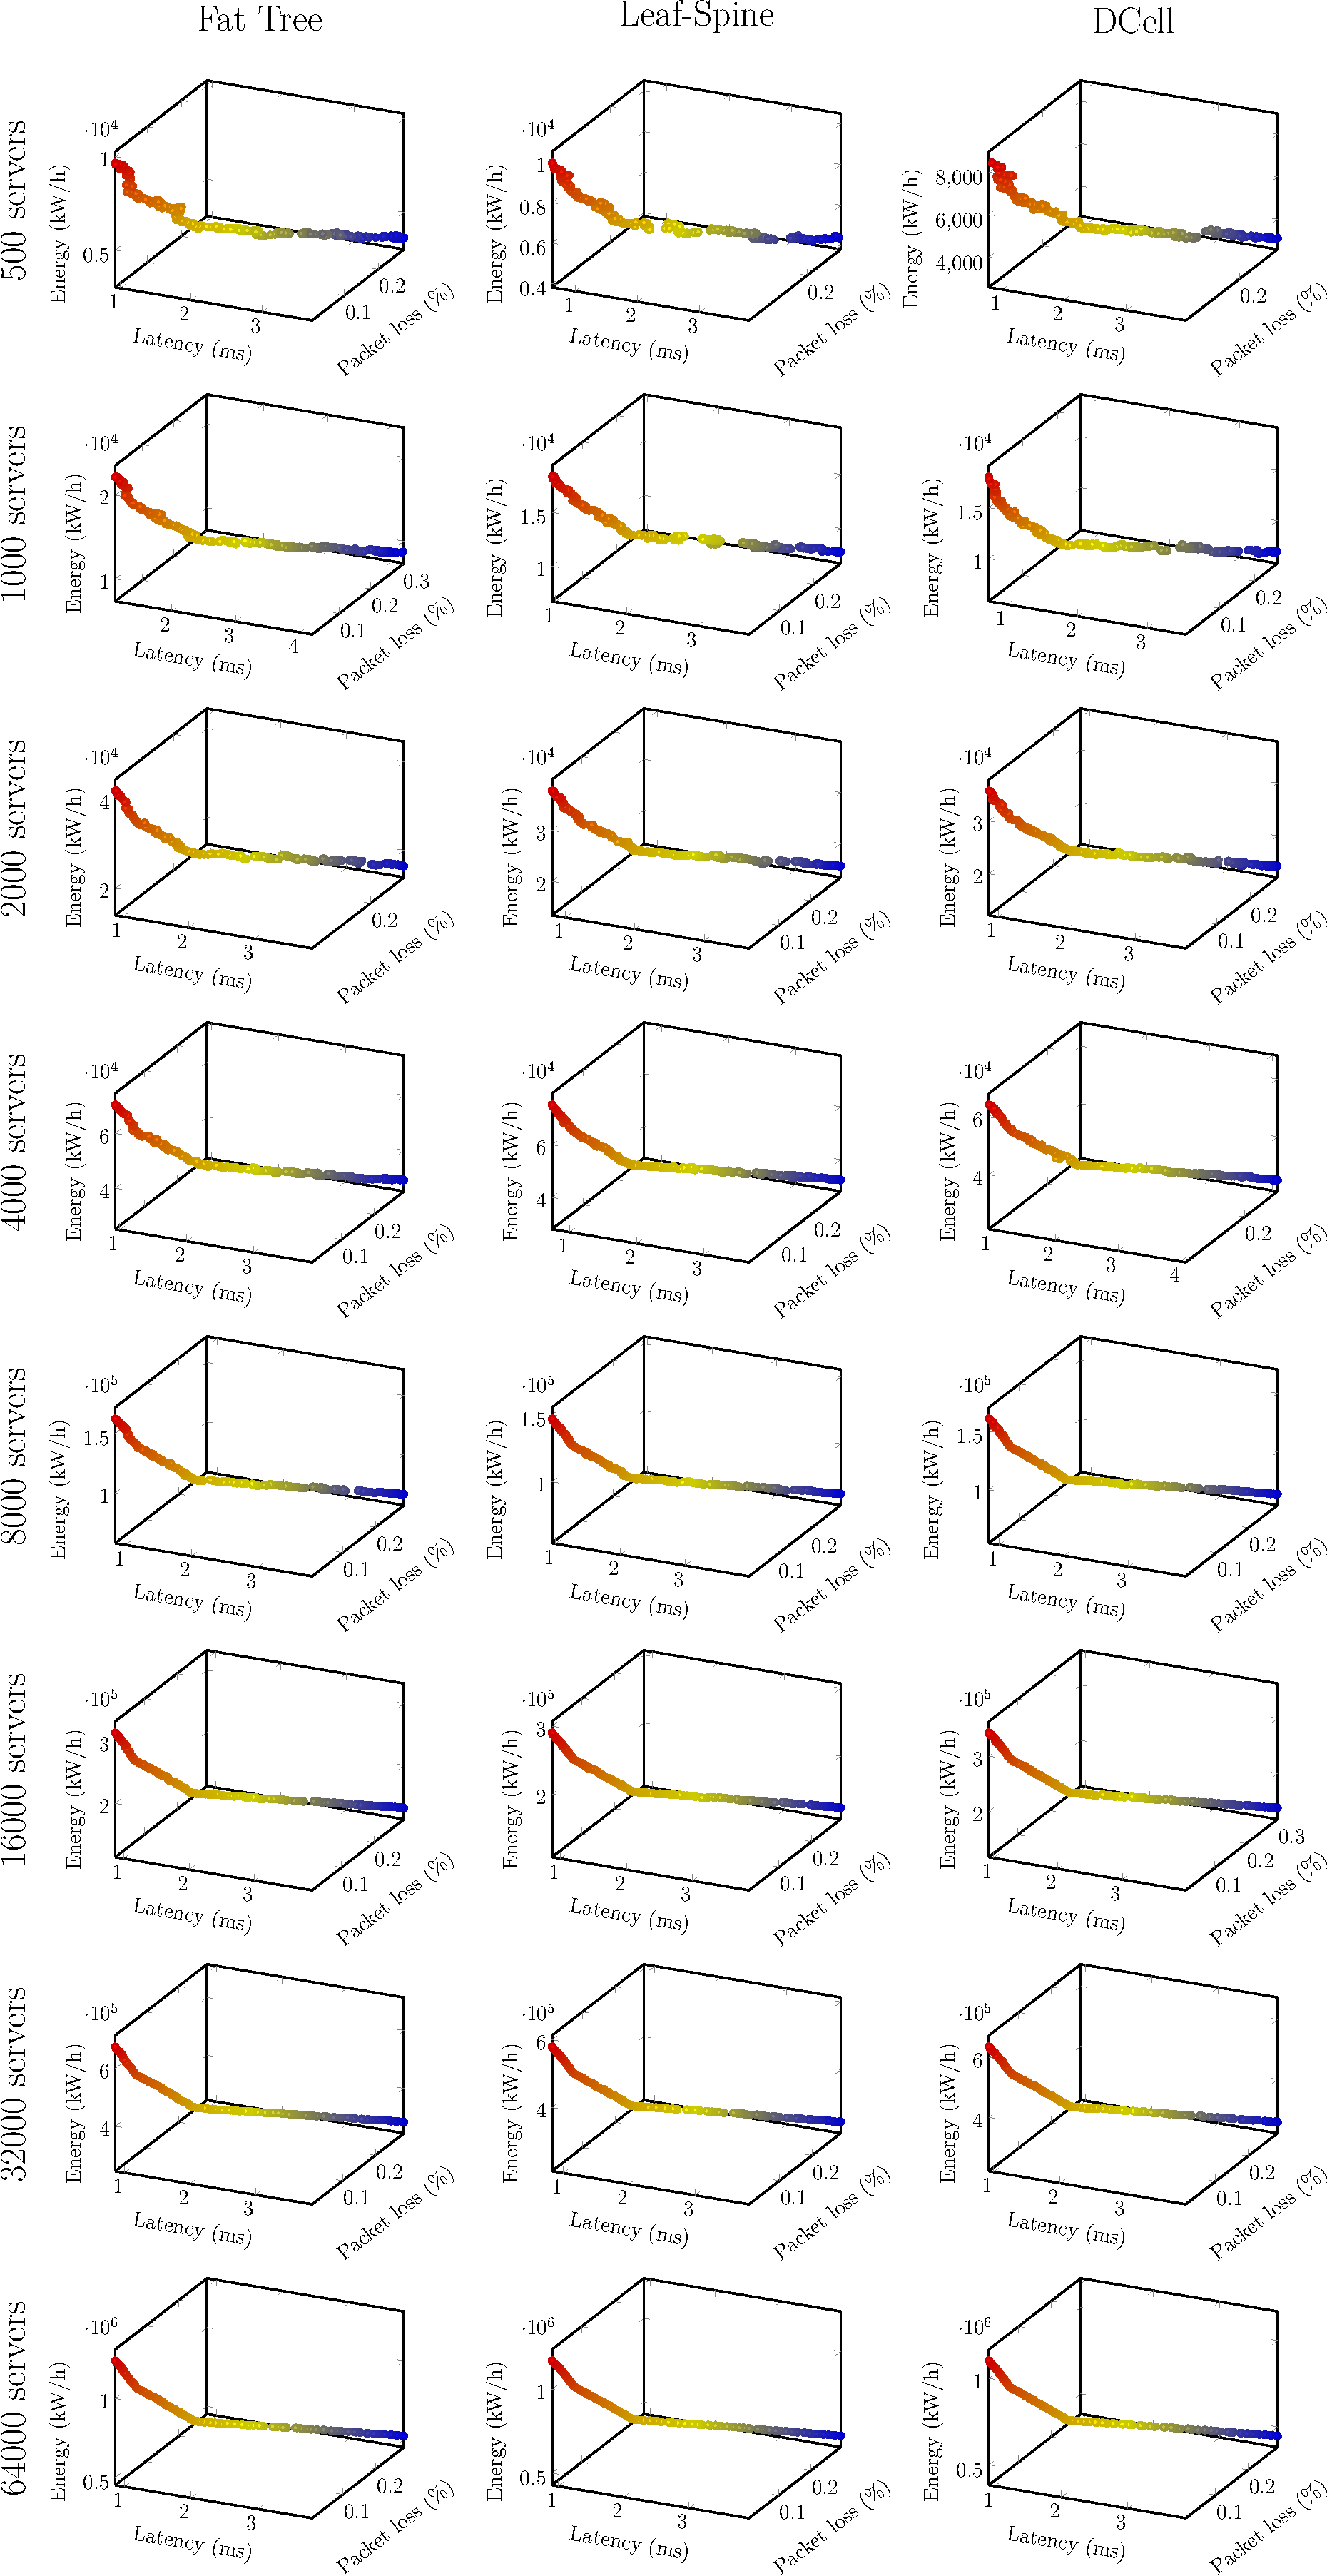
\includegraphics[width=\linewidth]{figures/graphs/models/pareto_fronts-crop}
    \caption{An illustrative example of the non-dominated solutions found by our proposed heuristic and both accurate models for problems with 16,000 servers.}
    \label{fig:models_pfs}
\end{figure}
\begin{figure}[t]
    \centering
    \begin{subfigure}[b]{0.9\linewidth}
        \includegraphics[width=\textwidth]{figures/graphs/models/fat_tree_hv-crop}
        \caption{Fat Tree}\vspace{.5em}
    \end{subfigure}
    \begin{subfigure}[b]{0.9\linewidth}
        \includegraphics[width=\textwidth]{figures/graphs/models/leaf_spine_hv-crop}
        \caption{Leaf-Spine}\vspace{.5em}
    \end{subfigure}
    \begin{subfigure}[b]{0.9\linewidth}
        \includegraphics[width=\textwidth]{figures/graphs/models/dcell_hv-crop}
        \caption{DCell}
    \end{subfigure}

    \caption{The median and quartiles of the normalized HV using our proposed algorithm and each model.}
    \label{fig:model_hv}
\end{figure}

\begin{table}
    \caption{Median wall clock time (s) as a multiple of the median wall clock time of our proposed model averaged over all topologies.}
    \label{tbl:model_time_multiple}

    \centering

    \resizebox{\columnwidth}{!}{%
        \begin{tabular}{lllllll}
            \toprule
            \multirow{2}{4em}{Model} & \multicolumn{6}{c}{Number of servers}                                       \\
            \cmidrule{2-7}
                                     & 500                                   & 1000  & 2000  & 4000 & 8000 & 16000 \\
            \midrule
            Accurate                 & 53.33                                 & 13.33 & 12.50 & 8.88 & 6.08 & 4.37  \\
            M/M/1/K                  & 20.00                                 & 5.33  & 5.07  & 3.80 & 2.80 & 2.23  \\
            M/M/1                    & 1.00                                  & 0.40  & 0.57  & 0.65 & 0.59 & 0.52  \\
            RU                       & 10.00                                 & 2.00  & 2.00  & 1.45 & 1.04 & 0.79  \\
            PLUS                     & 1.00                                  & 0.10  & 0.04  & 0.20 & 0.21 & 0.25  \\
            CWTPL                    & 10.00                                 & 2.67  & 2.43  & 1.60 & 1.13 & 0.85  \\
            \bottomrule
        \end{tabular}%
    }
\end{table}

Overall, the utilization heuristic presents a viable trade off between wall clock execution time and solution quality. Whilst some of the other heuristic approaches require less time still, the impact on solution quality and diversity is too severe. The proposed heuristic is likely better suited for larger problem instances where the execution time of more accurate models could be prohibitively time consuming.

\subsection{Applications to Large Data Centers}
\subsubsection{Methods}
Finally, to fully understand the scalability of our algorithm, we combined the most effective components as measured in previous tests and applied the resultant algorithm to increasingly large problem instances. Specifically, we integrated the utilization model, with our proposed operators and compression techniques into our proposed algorithm. Our aim is to identify which, if any, of these components prevent the algorithm from being applied to arbitrarily large VNFPPs.

We generated 30 problem instances for each topology and for increasingly large data center scales. Since solving a large problem instance can become time consuming, each data center scale contains approximately twice as many servers as the previous scale (i.e. $500$, $1000$, $2000$, $\dots$). We allowed the algorithm to run until it had performed 12,000 evaluations. We terminated testing when it was no longer practical to solve problem instances. For each problem we recorded the wall-clock execution time and calculated the HV of the final population.

% \begin{figure*}[p!]
%     \center
%     \includegraphics[width=\textwidth, height=.94\textheight, keepaspectratio]{figures/graphs/large_scale/pareto_fronts}
%     \caption{An illustration of the final populations found by our proposed algorithm on each topology.}
%     \label{fig:large_pf}
% \end{figure*}

\begin{figure*}[t]
    \includegraphics[width=\linewidth]{figures/graphs/large_scale/large_scale_hv}
    \caption{Hypervolume values for each topology and scale}
    \label{fig:large_hv}
\end{figure*}
\begin{figure}[t]
    \includegraphics[width=\linewidth]{figures/graphs/large_scale/large_scale_times}
    \caption{Wall clock execution time for each topology and scale}
    \label{fig:large_times}
\end{figure}

\subsubsection{Results}
\pref{fig:large_hv} demonstrates the high scalability of our algorithm. Specifically, our proposed algorithm can solve problems with up to 64,000 servers. We found that the routing table construction step prevented our algorithm from scaling to larger scale problems. The BFS based routing table construction algorithm has a low theoretical quadratic time complexity that scales with the number of components. In practice, a quadratic time complexity is unsuitable for very large topologies with hundreds of thousands of physical components. By way of illustration, we applied the routing construction algorithm to the first 1/10th of the servers in a DCell network topology with $\sim$128,000 servers. The construction of these routing tables took $\sim$124 hours ($\sim$5 days). By extrapolation, we can calculate the full construction of the routing tables would require at least 7 weeks to complete. Notably, unless otherwise resolved, this limitation applies to other optimization algorithms, including heuristics, that place VNFs in arbitrary networks.

As \pref{fig:large_times} shows, the other components of the algorithm demonstrated promising results on large scale topologies. Once preprocessing was complete, the algorithm execution time required on the order of seconds to minutes for 500-32000 servers. The largest data center topologies had a median time complexity of between $\sim$27 minutes (Leaf-Spine, 1631 seconds) and $\sim$70 minutes (DCell, 4225 seconds). 

It is interesting to note that the average execution time of the algorithm is significantly higher on the DCell topology. This could be explained by differences in the availability of cached resources. Whilst the data center is small, a larger proportion of the required memory can be held in a cache. However, on larger problems, \textit{cache prediction} will become more important. Cache prediction algorithms aim to retrieve data before it is requested. One assumption in cache prediction is the principle of spatial locality: the assumption that future memory accesses are likely to occur near to recent ones \cite{KennedyM92}. Since the DCell network topology allows servers with distant IDs to communicate, this assumption will be violated, and memory accesses are less likely to use a cache. In contrast, on the Fat Tree and Leaf-Spine topologies, nearby servers have similar IDs and hence are stored nearby in memory.

\pref{fig:large_hv} also shows that the initialization operator produces populations that are competitive with those found by our metaheuristic and hence could function as a standalone heuristic. It is clear from the results of earlier tests that the initialization operator is very effective as it is considers both the number of instances (through the improved initialization operator) and their placement (through our genotype-phenotype solution representation). Overall, our metaheuristic produces populations with a higher median HV, but the overall results are not significantly better than the initial population ($p < 0.05$) in any test case. Further, the initialization operator is a simpler algorithm, has a low time complexity and does not need to evaluate solutions. As a result, it is significantly faster on all problem instances. Despite this, since the initialization operator relies on the genotype-phenotype solution representation, it cannot scale to solve larger problem instances than our proposed algorithm.

The good relative performance of the initialization operator can be partly explained by the difficulty of very large problem instances. The largest problem instances in our tests contain on the order of 6000 services. Since the objective functions calculate the mean QoS across all services, a visible improvement to the objective functions requires improving the QoS of many services. However, the optimization algorithm is permitted only 12,000 evaluations to ensure it finishes in an acceptable time. As a result there is little opportunity to find improving solutions for many services. Irregardless, the effectiveness of the initialization operator should not be overlooked as it presents a viable alternative to more complex metaheuristic or exact approaches on very large problem instances.